\documentclass{article}
\usepackage[utf8]{inputenc}
\usepackage[spanish]{babel}
\usepackage{graphicx}
\usepackage{dirtytalk}
\usepackage{caratula}
\usepackage{enumerate}
\usepackage{amssymb}
\usepackage{amsmath}
\usepackage{geometry}
\usepackage{fixltx2e}
\usepackage{wrapfig}
\usepackage{cite}
\usepackage{float}
\usepackage[space]{grffile}
\geometry{
 a4paper,
 total={210mm,297mm},
 left=30mm,
 right=30mm,
 top=30mm,
 bottom=30mm,
 }
\begin{document}
% Estos comandos deben ir antes del \maketitle
\materia{Métodos Numéricos} % obligatorio

\titulo{Recuperatorio del Trabajo Práctico 3}
\subtitulo{También conocido como: por favor que se termine ya}
\grupo{
En este informe se presenta la implementación, desarrollo y análisis de resultados usados en la resolución de un problema práctico, con las herramientas estudiadas y provistas por la materia. El mismo consiste en agrandar una imagen por un cierto factor $k$.
Palabras Clave: Vecinos Más Cercanos, Interpolación Bilineal, Interpolación por Splines, Zoom\\}

\integrante{Bayardo Julián}{850/13}{julian@bayardo.com.ar} % obligatorio
\integrante{Carrasco Manuel}{646/13}{mgcarrasco2012@gmail.com} % obligatorio 
\integrante{Cuneo Christian}{755/13}{chriscuneo93@gmail.com} % obligatorio 
\integrante{Gómez Fabián}{799/13}{fabiandagomez@hotmail.com} % obligatorio 
\integrante{Keegan Maureen}{761/13}{maukeegan@hotmail.com} % obligatorio 

\maketitle

\pagebreak

\tableofcontents

\pagebreak

\section{Introducción Teórica}

Sea una función $F: \mathbb{R} \to \mathbb{R}$ desconocida, y un conjunto de datos ordenado: $$D = \{(x_0, F(x_0)), ..., (x_{n-1}, F(x_{n-1}))\} \text{ donde } x_i < x_{i+1} \forall i \in \{0, .., n-2\}$$
Supongamos que precisamos interpolar a $F$ por una función $f: [x_0, x_{n-1}] \to \mathbb{R}$. Concretamente, buscamos que $f(x_i) = F(x_i) \forall i \in \{0, .., n-1\}$; además, buscamos que $f$ de alguna forma logre generalizar bien, que logre parecerse a $F$ inclusive cuando la evaluemos en nuevos puntos que no estén en $D$. En la teórica vimos varios métodos para poder encontrar esta $f$ de forma tal que cumpla distintas propiedades según la metodología, pero en este trabajo nos limitaremos a utilizar dos de los métodos: la interpolación lineal, y la interpolación por splines.

El primero de estos métodos, la interpolación lineal, consiste en ampliar la clásica idea de buscar una recta que interpole a dos puntos: supongamos que tenemos dos puntos $\{(x_0, y_0), (x_1, y_1)\}$, entonces, y si suponemos que la relación entre ellos es $y(x) = mx + b$, podemos encontrar $m = \frac{y_1 - y_0}{x_1 - x_0}$ y $b = y_0 - m x_0$ como la única recta que pasa por ambos puntos. Supongamos, entonces, que tenemos nuestro conjunto $D$ descripto anteriormente, y tomamos la función

$$f(x) = \sum_{i=0}^{n-3} g_i(x) I_{[x_i, x_{i+1})}(x) + g_{n-2}(x) I_{[x_{n-2}, x_{n-1}]}(x)$$

Donde tenemos a $g_i$ como la función que evalúa a $x$ en la recta que interpola a $x_i$ con $x_{i+1}$:

$$g_{i}(x) = \frac{F(x_{i+1}) - F(x_i)}{x_{i+1} - x_i} (x - x_i) + F(x_i)$$

Y a $I$ como la función indicadora, que dado un conjunto $A$:

$$I_A(x) =
    \begin{cases}
        1 & \quad \iff x \in A\\
        0 & \quad \text{caso contrario}
    \end{cases}$$
    
Nótese que la función $f$ descripta toma el valor de la recta que interpola a $x_i$ con $x_{i+1}$ en los puntos que pertenecen al intervalo correspondiente.

\begin{wrapfigure}{r}{5.5cm}
\caption{Ejemplo de interpolación lineal para $F = sin$}\label{wrap-fig:1}
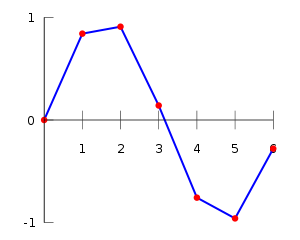
\includegraphics[width=5.5cm]{LinearInterpolationSine.png}
\end{wrapfigure} 


Observemos, además, que cuantos más puntos tengamos, mejor va a ser la aproximación a la función final $F$. Imitando la idea de la integral de Riemann, donde aproximando por rectángulos de base tendiendo a cero obtenemos el área debajo de la curva, intuitivamente si tuviésemos puntos con una distancia entre ellos tendiendo a cero, tendríamos también una aproximación óptima a la función por medio de una "interpolación lineal".

La próxima idea es la del uso de splines. La diferencia con respecto a la interpolación lineal es que ahora buscaremos interpolar por una secuencia de polinomios de grado 3 con ciertas propiedades específicas en lugar de una secuencia de rectas. De forma similar al caso anterior, tenemos

$$f(x) = \sum_{i=0}^{n-3} g_i(x) I_{[x_i, x_{i+1})}(x) + g_{n-2}(x) I_{[x_{n-2}, x_{n-1}]}(x)$$

Pero esta vez, vamos a pedir más restricciones sobre los polinomios fuera de la restricción natural de $f(x_i) = F(x_i) \forall i \in \{0, .., n-1\}$, pedimos que $\forall i \in \{0, .., n-2\}$:

\begin{itemize}
\item $g_i(x_{i+1}) = g_{i+1}(x_{i+1})$
\item $g'_i(x_{i+1}) = g'_{i+1}(x_{i+1})$
\item $g''_i(x_{i+1}) = g''_{i+1}(x_{i+1})$
\end{itemize}

Es importante destacar que esto no nos determina unívocamente al polinomio de grado 3 correspondiente, sino que nos permite tomar una familia de polinomios que particularmente cumplen que van a ser continuos cuando "los peguemos" en la $f(x)$. Es decir, son las condiciones suficientes para poder demostrar que la función de salida $f(x)$ es continua en todos los puntos de interés. Esto significa que necesitamos condiciones extra que nos permitan determinar unívocamente el polinomio que buscamos; a estas se las denomina "condiciones de borde". En la clase vimos 2 de estas condiciones:

La primera, el spline natural, consiste en pedir que $f''(x_i) = 0 \forall i \in \{0, n\}$.
La segunda, el spline sujeto, pedimos $f'(x_i) = F'(x_i) \forall i \in \{0, n\}$.

\section{Desarrollo}

$\ $ $\ $ $\ $ $\ $Implementamos tres métodos para hacer "zoom" de imágenes: vecino más cercano, interpolación bilineal, e interpolación por splines. En principio, el programa toma por parámetro una imagen en escala de grises $A \in \mathbb{Z}_{256}^{m \times n}$ y un factor $k \in \mathbb{N}_{>0}$ que indica cuánto extenderemos la imagen; concretamente, definimos una familia de transformaciones $f_k : \mathbb{Z}_{256}^{m \times n} \to \mathbb{Z}_{256}^{(k+1)(m-1)+1 \times (k+1)(n-1)+1}$ tal que:

$$(f_k(A))_{i, j} =
    \begin{cases}
        A_{\frac{i - 1}{k + 1} + 1, \frac{j - 1}{k + 1} + 1} & \quad \iff i \equiv 2 (\text{mod} k+1) \wedge j \equiv 2 (\text{mod} k+1) \\
        g_k(A, i, j) & \quad \text{caso contrario}
    \end{cases}$$

Donde $g_k$ es una transformación dependiente del método de interpolación que utilicemos. En concreto, el algoritmo consiste en aplicar la transformación $f_k$ con distintas $g_k$. Para que esta transformación realmente resulte en el efecto visual deseado, queda claro que precisamos de requerimientos muy específicos en términos de qué debería hacer la transformación; a modo de ejemplo, una transformación $g_k(A, i, j) = 0$ nos dejaría una imagen negra en todos los píxeles que no fueran los originales escalados. Para el efecto de agrandar la imagen en particular, queda claro que necesitamos de alguna forma que los píxeles determinados por $g_k$ tengan un sentido estético bien definido: que logren dar una continuidad a los objetos, a fines de que parezcan más grandes. La idea es que al interpolar los píxeles de la imagen real, podemos dar este efecto de continuidad en la nueva imagen.

En el primer método, la idea es que dado un píxel para el que queremos determinar su valor, los píxeles adyacentes en la imagen deberían proveer una buena aproximación al valor que debería tener el píxel realmente. En concreto, el algoritmo se fija cuál es el color del píxel más cercano al que estamos intentando determinar, y pone como valor el resultado de esta comparación. Observemos que podríamos encontrar casos en los que hayan múltiples píxeles a la misma distancia, por lo que debemos determinar cuál de estos valores tomar. En este caso, optamos por tomar la intensidad que se produzca con mayor frecuencia: notemos que $256 = 16 * 16$, es decir, podríamos dividir las posibles intensidades en 16 intervalos de 16 elementos (del 0 al 15, del 16 al 32, etcétera); por lo tanto, en el caso en que tengamos que hay más de un píxel a la misma distancia del punto central, podríamos tomar el punto cuyo intervalo correspondiente es el más frecuente. De cualquier forma, observemos que este criterio también podría fallar, en este caso, optamos por simplemente elegir el primer vecino más cercano descubierto.

En concreto, esperamos que este algoritmo genere imágenes que tiendan a mantener niveles similares de intensidad: los primeros dos criterios de alguna forma nos garantizan dos cuestiones: la primera, que vamos a mantener la intensidad muy fuertemente de forma local, ya que el hecho de elegir vecinos nos garantiza que todos los píxeles en la imagen final van a ser "parecidos"; la segunda, que los niveles de intensidad se van a mantener a nivel global, ya que vamos a tender a replicar los intervalos de mayor frecuencia en la imagen.

El segundo método, la interpolación bi-lineal, es ligeramente más complicado que el anterior: consiste en elegir una $g_k$ que nos permita hacer dos rondas de interpolaciones. La primera etapa interpolando dentro de cada una de las filas a los píxeles de la imagen original; observemos que si tomamos el índice $j$ en una de las filas, y el índice $l = j + 1$, ambos mapean en la nueva imagen de forma tal que están separados por $k$ píxeles: si entonces tomamos a $j'$ y a $l'$ como los índices anteriores en la nueva imagen, podemos encontrar una recta que pase por los valores $(j', A_{i, j})$ y $(l', A_{i, l})$. Nótese que esta recta posee dos propiedades interesantes: en primer lugar, todos los índices naturales entre $j'$ y $l'$ pertenecen al dominio; en segundo lugar, la imagen de la recta toma valores que interpolan a los valores de la matriz original, por lo que intuitivamente estamos generando un degradé de la intensidad de la imagen, convirtiendo la intensidad de un punto en la intensidad de otro. 

Habiendo encontrado esta recta, podemos determinar la intensidad de los píxeles en la fila $i$, de las columnas $j'$ a $l'$ como los valores de la recta interpoladora redondeados a enteros. Repetir este proceso para todos los valores de $j$ hasta el $n - 1$, y para todos los valores de $i$ nos crearía una imagen con todas las filas que ya estaban en la imagen original llenas de valores de intensidad, y tan sólo faltaría completar las $k$ columnas vacías que se generan entre cada fila. Pero observemos que podemos llevar a cabo este mismo proceso entre cada una de las columnas, generando la imagen completa.

Es fácil darse cuenta que la imagen nueva mantendrá los niveles de luminosidad de la imagen inicial, ya que todo el tiempo estaremos interpolando por rectas, que no nos permitirán salirnos de rango y terminar saturando los valores. Además, sería esperable que obtengamos mayores discrepancias en las columnas completamente agregadas por el método de interpolación (en el ejemplo, las columnas con índices entre $j'$ y $l'$), ya que estas habrán sido creadas enteramente a través de aproximaciones lineales. Conjeturamos, también, que probablemente este método introduzca un menor error que el primero, ya que el primer algoritmo probablemente genere una idea de discontinuidad en la frontera del radio afectado por un píxel: eventualmente se debe pasar de un vecino a otro, y ese efecto no coincide con la experiencia sensorial, que da más una sensación de suavidad entre los colores. A pesar de esto, estimamos que este método va a tener problemas en términos más globales, ya que un degradé no necesariamente es la forma en la que los objetos se encuentran delimitados en la vida real; a modo de ejemplo, imaginemos un escritorio de madera con una pared blanca de fondo: los bordes del escritorio van a tener una transición de color abrupta, una especie de discontinuidad, mientras que las partes íntegramente de madera van a tener una transición más suave, o de degradé entre los valores de luminosidad.

El tercer método, la interpolación por splines, consiste en aumentar la complejidad del método anterior: en lugar de considerar interpolaciones lineales entre dos píxeles, tomamos polinomios que interpolen de a $l$ píxeles. El sentido está en pedir que los mismos cumplan las características de spline definidas antes, que nos permitirán afirmar no sólo que interpolan a los puntos requeridos, sino que además preservan la idea de continuidad de la intensidad. Más aun, al ser polinomios que tomen tanta información en cuenta, también harán una mejor transición en los bordes de los objetos, que nos representa una mejoría visual con respecto a la interpolación lineal del método anterior. La particularidad de que interpolen de a $l$ píxeles es por una propiedad fundamental de los splines: observemos que los valores de las derivadas en las puntas (los que hacen la distinción entre el spline natural y el spline sujeto) dependen del tipo de spline que busquemos, y por lo tanto no es lo mismo si consideramos que las puntas son el primer y último píxel de la imagen o si la dividimos de alguna forma. En concreto, los $l$ píxeles nos permiten dividir la imagen en cuadrados de $l \times l$, y crear splines entre los píxeles del medio, tomando los bordes como compartidos.

\section{Implementación}

Para simplificar la comprensión, dentro de la carpeta de experimentación se encuentran las carpetas bilineal, knn y splines, correspondientes a los resultados experimentales; y originales, correspondiente a las imágenes que utilizamos. Además, tenemos una copia idéntica dentro de la carpeta bigimages, que juegan los mismos roles pero con imágenes mucho más grandes.

Para poder compilar, utilizamos el script de python proveeido por la cátedra; la metodología no varía. En tanto a replicar los experimentos, cada una de las carpetas con experimentos tiene un archivo \texttt{runner.sh}, que se ocupa de correr los experimentos y generar las estadísticas. Luego, correr el script \texttt{producer.py} se ocupa de generar las mediciones de error y de producir un archivo de salida con formato csv que resume toda la información, así como de generar archivos csv que guardan el error punto a punto de las imagenes. Es muy importante tener en cuenta que correr estos scripts para la carpeta bigimages resulta en una gran cantidad de archivos de tamaños muy grandes, totalizando unos 20GB de espacio, sin mencionar el tiempo de cómputo requerido, así que recomendamos tomar la precaución de tener el espacio disponible antes de intentar reproducir los resultados.

Finalmente, este archivo de salida se utiliza como entrada para Tableau, el software graficador. Los archivos de Tableau para generar todos los gráficos mostrados, e inclusive algunos más utilizados como referencia para entender mejor el problema, se encuentran en los archivos \texttt{.twb}.

\subsection{Splines}

Para la implementación de splines, creamos una clase Trazador Cúbico y la utilizamos para encapsular tanto el cálculo de los coeficientes como la evaluación en un punto. Para encontrar dichos coeficientes, fue necesario resolver un sistema de ecuaciones, por lo que incluimos la clase Matriz usada en el trabajo práctico anterior, e implementamos un algoritmo de Eliminación Gaussiana optimizado para el problema en particular. Vimos que la matriz a triangular sólo efectuaba una operación por columna (ya que el resto de las posiciones son nulas) y por lo tanto nos pareció mejor adaptar el algoritmo a esta situación, para no perder eficiencia en este punto. También optamos por aplicar el trazador cúbico natural, es decir optamos por tomar $S_{0}''(x_{0})= S_{n-1}'' (x_{n}) = 0$ , siendo $S_{j}$ el polinomio de grado menor o igual que 3 en $[x_{j},x_{j+1}] \forall i \in \{0, n-1\}$.

La implementación por splines toma un parámetro extra que el resto de los algoritmos no toma. Este parámetro representa el tamaño de bloque en el cual se realizará el spline. Es decir con cuántos píxeles se procesará el trazador. Una vez tomado el bloque, se actúa como si fuese una subimagen y se le aplica zoom. En el siguiente gráfico se muestra como quedarían los bloques armados para una configuración determinada. Se ve como cuando el tamaño de la imagen no llega a completar los bloques necesarios para que todo píxel pertenezca a un bloque, se utilizan más bloques pero repitiendo píxeles entre ellos.

\begin{figure}[H]
\centering
  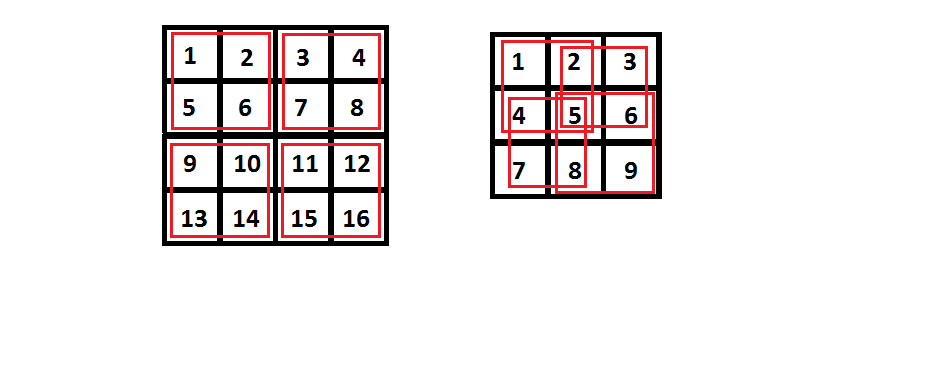
\includegraphics[scale=0.7]{Bloques}
  \caption{Bloques}\label{fig:Bloques}
\end{figure}

Para este método corroboramos su funcionamiento para dos casos simples de zoom con splines.

El primero consistió en una pequeña imagen de 4x4 pixeles en la que todos tenían el mismo valor. Efectivamente luego de ser procesada, el output mantuvo los valores en los pixeles nuevos.

El segundo caso consistió  en evaluar como funcionaba la interpolación en filas. La imagen nuevamente fue de 4x4 pixeles en donde cada fila tenia los valores: 1 3 5 7
El zoom se efectuó con k=1 y B=4, la fila resultante fue: 1,2,3,4,5,6,7

El output fue verificado con matlab. Estos tests de implementación se encuentran adjuntos con el trabajo.

\subsection{Vecinos más cercanos}

La idea del algoritmo es simple: buscar los vecinos más cercanos del píxel a estimar, y luego decidir mediante cierta condición cuál de estos elegir como valor para el nuevo píxel. En un principio, para cada nuevo píxel calculamos su distancia con todos los píxeles con valores conocidos, y luego nos quedamos con aquellos que tenían la distancia mínima. Esto afectaba seriamente el tiempo de ejecución, ya que para cada nuevo elemento en la imagen se hacían n cantidad de operaciones, siendo n el tamaño original de la imagen. Para intentar disminuir este costo, analizamos los distintos casos de posibles ubicaciones de los nuevos píxeles:
\begin{itemize}

\item El píxel se encuentra en una fila (o columna) que contiene píxeles cuyos valores son conocidos. Para k par, todos los píxeles tienen un sólo vecino más cercano. Para k impar, en cambio, podemos ver en el gráfico que en el peor caso debemos considerar dos vecinos y luego desempatar a través de la condición elegida.

\begin{figure}[H]
\begin{center}
  
\includegraphics[scale=0.25]{vecinos1}
  \caption{El píxel se encuentra en una fila (o columna) que contiene píxeles cuyos valores son conocidos.}\label{fig:vecinos1}
\end{center}
\end{figure}


\item El píxel se encuentra en una fila (o columna) que no contiene píxeles con valores conocidos. De forma análoga al caso anterior, para k par todos los píxeles tienen un sólo vecino más cercano. Sin embargo, para k impar, en el peor caso debemos considerar cuatro vecinos más cercanos.

\begin{figure}[H]
\begin{center}
  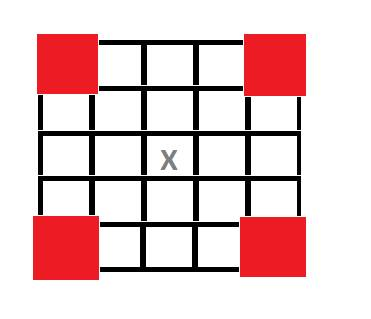
\includegraphics[scale=0.25]{vecinos2}
  \caption{El píxel se encuentra en una fila (o columna) que no contiene píxeles con valores conocidos.}\label{fig:vecinos2}
\end{center}
\end{figure}
\end{itemize}

De este modo optimizamos el algoritmo considerando siempre que nos encontramos en el peor caso, calculando sólamente 4 distancias, y, de ser necesario, desempatando con la condición elegida.

\section{Experimentación y Discusión}

\subsection{Razones detrás de la selección de imágenes}

A modo de poder experimentar con distintas composiciones de imágenes, decidimos utilizar 6 imágenes distintas: 2 imágenes de figuras geométricas, 2 imágenes de paisajes, y 2 imágenes con rostros de mujeres. Las mismas fueron buscadas en Deviant Art, de tamaños más grandes que el objetivo para asegurarnos de no introducir artifacts a lo largo del proceso, y reducidas con Matlab a un tamaño de $401\times401$.

La elección en particular de este tipo de imágenes, se debe a las grandes diferencias estructurales entre las distintas categorías. Con esto quisimos probar cómo se comportaban los distintos algoritmos con dos imágenes de cada tipo para ver si el método se podía adaptar a los distintos patrones de imágenes o solo para alguno$/$s de ellos. Las categorías se componen por : 
\begin{itemize}
\item GEOMÉTRICAS : Consta de dos imágenes con patrones bastante determinados que varían drásticamente de color y de dos formas distintas entre ellas.
\item PAISAJES : Imágenes sin patrones definidos con poco quiebre de color y áreas de color continuo o cambios suaves, con poco detalle apreciable. 
\item RETRATOS : Imágenes con detalles precisos y apreciables. 
\end{itemize}

\begin{figure}[H]
\minipage{0.32\textwidth}
  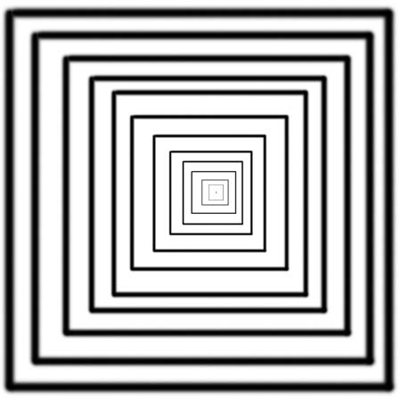
\includegraphics[width=\linewidth]{geometrica_1}
  \caption{Imagen Geométrica 1}\label{fig:geometrica_1}
\endminipage\hfill
\minipage{0.32\textwidth}
  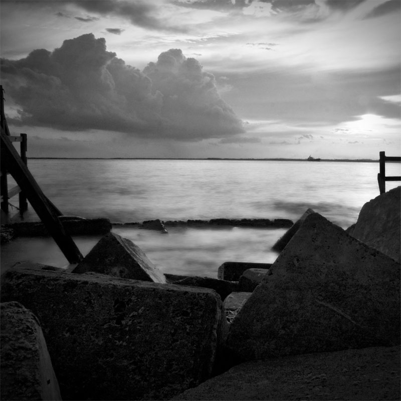
\includegraphics[width=\linewidth]{paisaje_1}
  \caption{Imagen Paisaje 1}\label{fig:paisaje_1}
\endminipage\hfill
\minipage{0.32\textwidth}%
  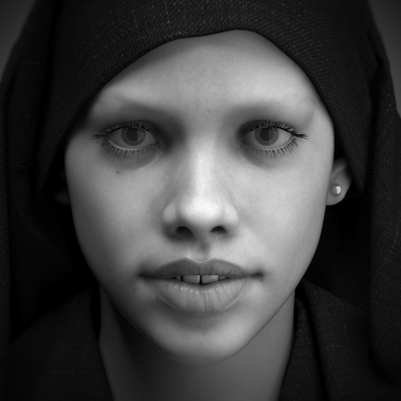
\includegraphics[width=\linewidth]{rostro_1}
  \caption{Imagen rostro 1}\label{fig:rostro_1}
\endminipage
\end{figure}

\begin{figure}[H]
\minipage{0.32\textwidth}
  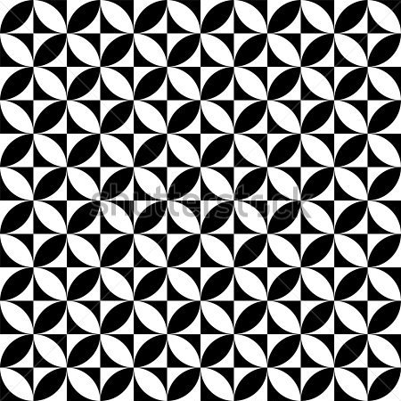
\includegraphics[width=\linewidth]{geometrica_2}
  \caption{Imagen Geométrica 2}\label{fig:geometrica_2}
\endminipage\hfill
\minipage{0.32\textwidth}
  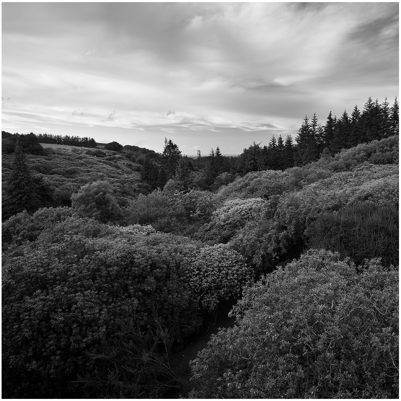
\includegraphics[width=\linewidth]{paisaje_2}
  \caption{Imagen Paisaje 2}\label{fig:paisaje_2}
\endminipage\hfill
\minipage{0.32\textwidth}%
  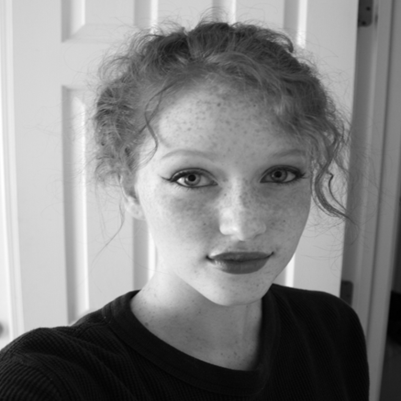
\includegraphics[width=\linewidth]{rostro_2}
  \caption{Imagen rostro 2}\label{fig:rostro_2}
\endminipage
\end{figure}

El tomar imagenes de $401\times401$ es una decisión ampliamente relacionada con los valores posibles de $K$. Nosotros buscábamos poder achicar las imágenes que ya teníamos y volver a extenderlas a su tamaño original para poder realizar mediciones de error. Observemos que dado un índice basado en 0 $(i, j)$ en una imagen de $n \times n$, el índice correspondiente en la imagen expandida es $(i', j') = (i (K+1), j (K+1))$. Es decir, si tomamos en particular el último índice $(i, j) = (n-1, n-1)$, las entradas correspondientes son $((n-1) (K+1), (n-1) (K+1))$, por lo que la imagen extendida es de $n' \times n'$ con $n' = (n-1) (K+1) + 1$. Entonces, si tomamos a $n' = 401$ tenemos que $(n-1)(K+1) = 400$, implicando que tanto $n-1$ como $K+1$ son divisores de $400$, por lo que $n-1, K+1 \in \{1, 2, 4, 5, 8, 10, 16, 20, 25, 40, 50, 80, 100, 200, 400\}$. Para medir la calidad de la interpolación, no nos interesa particularmente cómo se comportan los valores de $n-1$, sino que sólo nos importa variar $K+1$, diciéndonos entonces que $K \in \{0,1,3,4,7,9,15,19,24,39,49,79,99,199,399\}$ y $n = \frac{n'-1}{K+1} + 1$. Además, cabe destacar que tomar $K = 0$ es no hacer ningún cambio, por lo que fue descartado instantáneamente; fuera de eso, tomar valores de $K$ demasiado grandes pensamos que nos va a terminar distorsionando demasiado la imagen: para insertar $399$ píxeles, primero hay que disminuir la imagen a $2 \times 2$, efectivamente borrando cualquier dato que podamos tener. Finalmente, optando por la moderación, decidimos tomar

$$K \in \{1, 3, 4, 7, 9\}$$

Además, para el caso particular de splines, teníamos que elegir tamaños de bloque para utilizar. Elegimos utilizar $B \in \{4, 8, B'\}$, donde $B'$ es un valor dependiente de $K$, que nos permite tomar un bloque unitario, del tamaño total de la imagen reducida. El mismo está determinado por la relación

$$B' = \frac{400}{K+1} + 1$$

%%%%%% TODO: Hablar sobre la medición de tiempos
%% Y ACTUALIZAR ACA ABAJO

Intentamos incluir una cantidad de imágenes razonable, lo suficiente como para ilustrar los objetivos que buscamos. Sin embargo, debido a la naturaleza del trabajo, la cantidad de imágenes que realmente es necesario mirar para entender del todo qué es lo que decimos es bastante superior a las que consideramos prudente para un informe, por lo tanto, haremos ocasionalmente referencia a imágenes que están dentro de la carpeta experimentación, relacionadas con los resultados particulares que obtuvimos. 

\subsection{El error al interpolar}

Nuestra primer hipótesis era que la técnica de vecinos más cercanos iba a tener un mayor error cuadrático medio que la interpolación bi-lineal, y que esta última iba a tener un mayor error cuadrático medio que la interpolación por splines. Por supuesto, pensábamos que de cualquier forma el error (y la superioridad de una técnica por sobre la otra) iba a depender de la aplicación concreta que le diésemos: supusimos que la composición de la imagen iba a influir ampliamente en la efectividad de los algoritmos, y que muy probablemente la relación que establecimos fuese a romperse en algún caso particular.

Además pensábamos que, en general, utilizar tanto splines como kNN iba a ser consistentemente mejor que la interpolación bi-lineal en los casos donde la composición de la imagen fuera más rica en componentes, como los casos de los rostros y el paisaje, mientras que la interpolación bi-lineal se comportaría mejor en el caso de las figuras geométricas.

\begin{figure}[H]
\centering
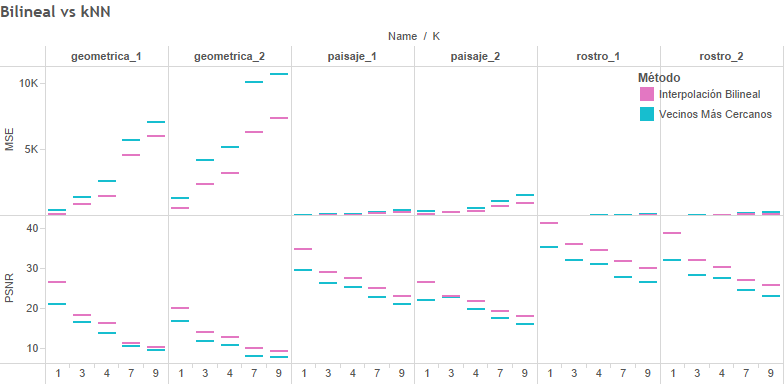
\includegraphics[width=17cm]{Bilineal vs kNN}
\caption{Mean Squared Error (valores más altos son mayor desigualdad entre las imágenes) y Peak Signal to Noise Ratio (valores más altos son mayor igualdad entre las imágenes) en función de la composición de la imagen y el valor de $K$, para los casos de interpolación bi-lineal y vecinos más cercanos.}
\label{fig:bilineal_vs_knn}
\end{figure}

Observemos que en la figura \ref{fig:bilineal_vs_knn} encontramos que para todas las composiciones testeadas el método de interpolación bi-lineal obtiene consistentemente mejores resultados. Nótese, además, que en las imágenes geométricas tenemos un error ampliamente más grande que en los otros casos; esto lo atribuimos a los posibles problemas en torno a los "bordes" presentes en la imagen: tenemos una mayor cantidad de discontinuidades, y mucho más abruptas que en los otros casos, haciendo que utilizar tanto un degradé como una votación de la mayoría resulte en elecciones problemáticas.

En términos de splines, es fácil ver en la figura \ref{fig:bilineal_vs_splines_geo} que los niveles de error son similares al caso anterior, y que ninguno de los dos métodos es consistentemente mejor que el otro para este tipo de composición. Además, el error entre los distintos tamaños de bloque no parece seguir ninguna relación concreta (en el sentido que no es consistente que siempre sea mejor tomar un tamaño de bloque igual al tamaño de la imagen, ni similares), por lo que en principio el tamaño de bloque no estaría generando grandes cambios desde el punto de vista del error.

Por otro lado, si observamos la figura \ref{fig:bilineal_vs_splines} encontramos una vez más que no tenemos una mejora consistente en ninguna de las composiciones, ni siquiera considerando distintos tamaños de bloques. Es decir, lo único que podemos concluir con seguridad es que definitivamente ambos algoritmos son mejores que utilizar vecinos más cercanos, ya que la efectividad de splines y bi-lineal es muy similar, y esta última es consistentemente mayor que la de kNN.

\begin{figure}[H]
\centering
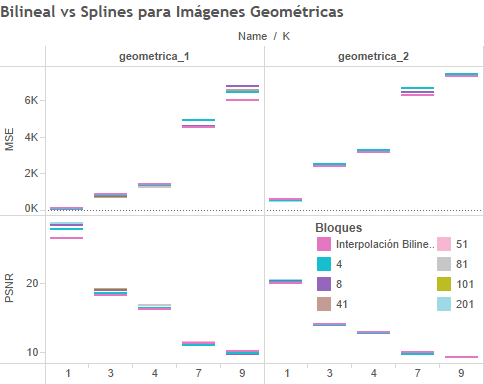
\includegraphics[width=10cm]{Bilineal vs Splines Geometricas}
\caption{Mean Squared Error (valores más altos son mayor desigualdad entre las imágenes) y Peak Signal to Noise Ratio (valores más altos son mayor igualdad entre las imágenes) en función de la composición de la imagen y el valor de $K$, para los casos de interpolación bi-lineal y splines.}
\label{fig:bilineal_vs_splines_geo}
\end{figure}

\begin{figure}[H]
\centering
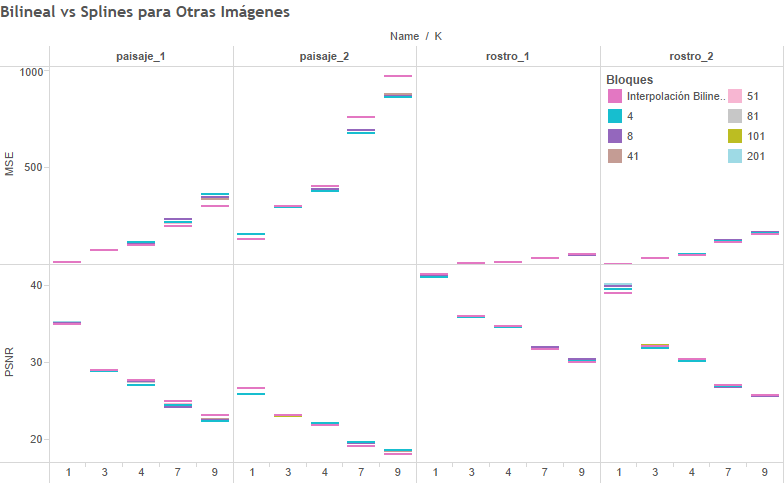
\includegraphics[width=14cm]{Bilineal vs Splines para Otras Imagenes}
\caption{Mean Squared Error (valores más altos son mayor desigualdad entre las imágenes) y Peak Signal to Noise Ratio (valores más altos son mayor igualdad entre las imágenes) en función de la composición de la imagen y el valor de $K$, para los casos de interpolación bi-lineal y splines.}
\label{fig:bilineal_vs_splines}
\end{figure}

\subsection{Las limitaciones de los algoritmos}

A modo de entender los problemas de los algoritmos propuestos, así como de intentar comprender la inesperada similitud entre la efectividad de los algoritmos de interpolación bi-lineal y con splines, decidimos buscar las raíces de los errores en las interpolaciones que ya habíamos realizado. En todos los casos tomamos las imágenes con mayor error del conjunto, que consideramos nos van a permitir ver mejor las falencias de los algoritmos. 

En principio, nosotros pensábamos que la limitación de kNN iba a radicar en los bordes de las figuras: que iba a tender a tener problemas en las zonas donde se intersequen colores demasiado distintos. Por otro lado, pensamos que bi-lineal iba a lograr una mejoría en estos términos, debido a su capacidad de utilizar degrades en los bordes. Finalmente, hipotetizamos que splines probablemente realice mejores transiciones aun que la interpolación bi-lineal. Debido a los resultados del experimento anterior, nos vemos forzados a pensar que el motivo de error en la interpolación con splines probablemente haya cambiado de eje.

Desde un punto de vista puramente cualitativo, es fácil ver que en el caso de la imagen geométrica 1 (puede verse la progresión en el archivo adjunto \texttt{Progreso Geométrica 1.jpg}) agrandar el valor de $K$ causa un decrecimiento muy rápido en la calidad de las imágenes: los resultados de $K=1$ son ampliamente aceptables, y casi no se discierne el efecto, mientras que ya saltando a $K=2$ se comienza a notar el efecto en los detalles; al llegar a $K=9$ los resultados casi no guardan similitud con la imagen original. Si observamos la progresión de imágenes correspondiente a kNN, puede verse el efecto en los cambios de color que habíamos mencionado anteriormente, así como también la mejoría de esta característica en las otras metodologías. Cabe destacar que en particular utilizar Splines cambia el color de fondo blanco de la imagen por un color gris en todas sus variantes.

Pensando de una forma más cuantitativa, en principio la visualización de la figura \ref{fig:error_geometrica_1} muestra que en la imagen de kNN hay consistentemente errores en los bordes, como habíamos observado anteriormente, y que además los errores tienden a ser muy fuertemente marcados. Pensamos que esto es consistente con la idea del algoritmo de elegir por votación de la mayoría: las lineas marcadas tan fuertemente tienen que ver con los limites de los conjuntos de vecinos. Por otro lado, la imagen correspondiente a interpolación bi-lineal tiende a tener bordes menos marcados, en forma de degradé, que también es consistente con los pensamientos que habíamos expuesto.

Sin embargo, cabe destacar que la diferencia es mucho menos marcada entre las variantes de splines y la interpolación bi-lineal; a pesar de que el caso de splines tienda a una mayor suavidad en los bordes de la figura, y que en general hay un menor nivel de error. Sospechamos que muy probablemente el causante de este problema sea el área entre los bordes: pensamos que el cambio de color que introduce la interpolación por splines genera una cantidad de error suficiente como para compensar.

\begin{figure}[H]
\centering
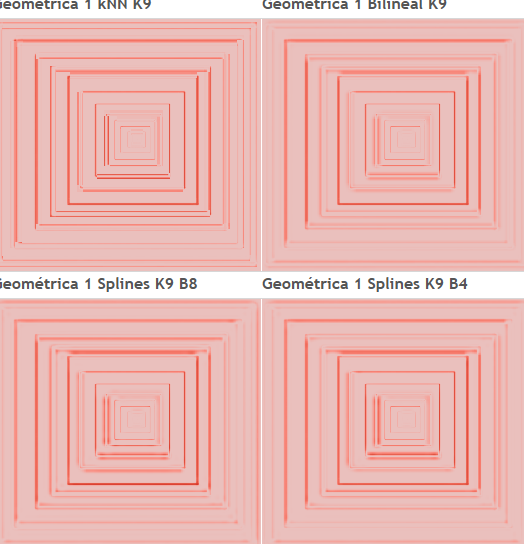
\includegraphics[width=10cm]{Error Geometrica 1}
\caption{Visualización del error en los puntos de la imagen, cada punto se corresponde con lo que aporta al MSE; todas las escalas están normalizadas. El rojo claro predominante suele ser 0, aunque hay pequeños cambios. Es importante tener en cuenta que dado el alto valor de $K$ que tomamos, es muy posible que la imágen reducida haya perdido algunas de las características que tenía inicialmente. No realizamos el error para splines con bloques unitarios por considerarlo poco ilustrativo.}
\label{fig:error_geometrica_1}
\end{figure}

A modo de aclarar esta cuestión, armamos la figura \ref{fig:zonas_error_geometrica_1}. Observemos que, tal como pensábamos, los problemas de la interpolación por splines se centran mayoritariamente en el área intermedia a los bordes, y esto es lo que genera los niveles de error tan similares a los de la interpolación bi-lineal. Sospechamos que el problema con los splines probablemente radique en la cantidad de bordes muy pequeños que posee la imagen original, así como en la dificultad de generar una recta constante (correspondiente al área gris entre medio de las rayas negras) utilizando un polinomio necesariamente de grado 3, como muestra la progresión de los colores en las áreas grises de las imágenes de splines, donde el color tiende a cambiar entre una y otra.

\begin{figure}[H]
\centering
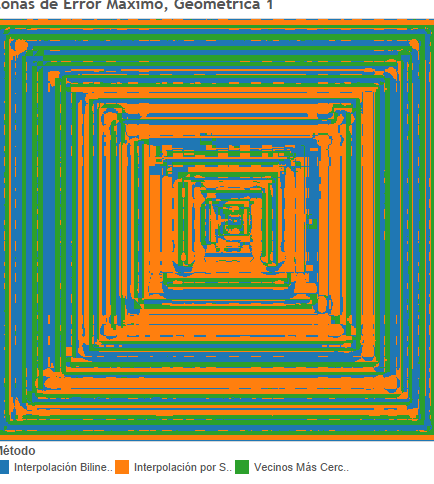
\includegraphics[width=9cm]{Zonas de Error Maximo Geometrica 1}
\caption{Zonificación del error en función del método, cuando $K=8$ y $B=9$. Cada píxel está coloreado según el método que más error alcanza en el lugar.}
\label{fig:zonas_error_geometrica_1}
\end{figure}

Continuando con los paisajes, la progresión (puede verse en el archivo adjunto \texttt{Progreso Paisaje 2.jpg}) muestra, en principio, que kNN tiende a oscurecer la imagen: como mencionamos en el desarrollo, los niveles de luminosidad se propagan a lo largo de la imagen, haciendo que áreas que anteriormente eran más claras se conviertan en oscuras. Un experimento interesante para continuar sería ver qué sucede con imágenes con distintos niveles de luminosidad. Además, es fácil ver cómo ya con $K=1$ en kNN se ha perdido una buena parte del detalle: los árboles se ven notoriamente peor, y la linea del horizonte tiene rasgos más endurecidos, en contraste con la fotografía original que era como más suave. Fuera de eso, es notorio como el borde de la imagen tiene pequeñas zonas en blanco que originalmente no estaban: esto se corresponde con la propagación del borde blanco que teníamos anteriormente.

En términos de la interpolación bi-lineal, observemos que la zona inferior izquierda de $K=1$ ha oscurecido, y se han perdido detalles en la misma; también se ha oscurecido la zona arbolada que linda con el horizonte, aunque en términos generales la imagen retiene muy bien las características iniciales. Observemos que el borde de la imagen se ha vuelto ligeramente más suave de lo que era originalmente. Por otro lado, la interpolación por splines no ha llevado a cambios sustanciales visibles. Es muy fácil ver una vez más que el aumento de $K$ tiende a empeorar en gran cantidad a la imagen, lo interesante es que las imágenes siguen manteniendo los rasgos generales de las versiones con $K$ más chicos: no hay grandes cambios en términos de la luminosidad, sino que sólo decrece la calidad.

Desde un punto de vista cuantitativo, sospechamos que muy probablemente la mayoría del error se concentraría en los cambios bruscos, fundamentalmente porque es donde los algoritmos parecerían tener más problemas; además, la imagen tiene una zona de intersección con el horizonte. Como vemos en la figura \ref{fig:error_paisaje_2}, efectivamente todos los métodos terminan mostrando una pequeña concentración de error donde estaría la intersección, correspondiente a los cambios en la arboleda que se ve al fondo de la imagen; también tenemos una franja de blanco en las esquinas de la imagen, causante de la concentración de error más fuerte que vemos, una vez más mostrando que los algoritmos tienden a tener problemas cuando hay grandes cambios de color en las imágenes. Observemos además que el resultado de kNN muestra muy claramente una cantidad de pequeñas zonas rojas distribuidas en la parte inferior, suponemos correspondiente a los cambios en luminosidad de los que hablábamos anteriormente.

\begin{figure}[H]
\centering
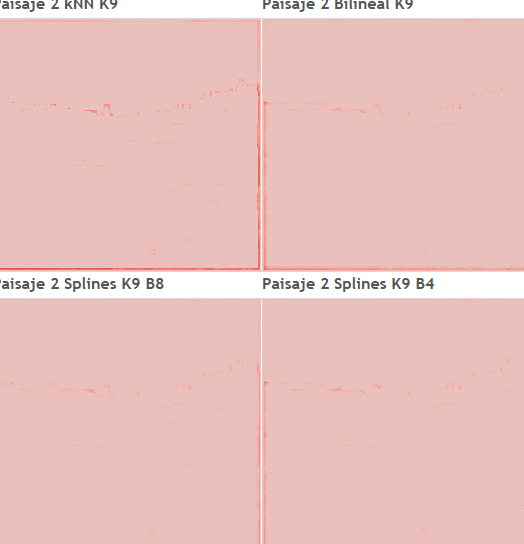
\includegraphics[width=10cm]{Error Paisaje 2}
\caption{Visualización del error en los puntos de la imagen, cada punto se corresponde con lo que aporta al MSE; todas las escalas están normalizadas. El rojo claro predominante suele ser 0, aunque hay pequeños cambios. No realizamos el error para splines con bloques unitarios por considerarlo poco ilustrativo.}
\label{fig:error_paisaje_2}
\end{figure}

En el último caso, el del rostro 2, observar la progresión (que una vez más puede verse en el archivo adjunto \texttt{Progreso Rostro 2.jpg}) muestra unos niveles muy superiores desde un punto de vista cualitativo: se logra una imagen bastante buena inclusive con $K=3$. Donde podemos ver que los primeros artifacts se comienzan a formar en la zona de los ojos y el pelo, y luego se propagan hacia la ropa, la puerta del fondo y el resto de los rasgos faciales. La figura \ref{fig:error_rostro_2} muestra como claramente el error más grande se sitúa en la nariz y la ropa. Observemos que el caso con menor error en general es una vez más el de splines, que evidentemente alcanza un mejor balance.

\begin{figure}[H]
\centering
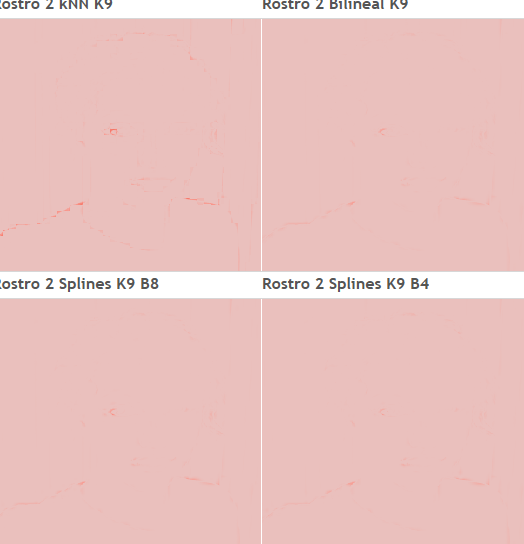
\includegraphics[width=10cm]{Error Rostro 2}
\caption{Visualización del error en los puntos de la imagen, cada punto se corresponde con lo que aporta al MSE; todas las escalas están normalizadas. El rojo claro predominante suele ser 0, aunque hay pequeños cambios. No realizamos el error para splines con bloques unitarios por considerarlo poco ilustrativo.}
\label{fig:error_rostro_2}
\end{figure}

En conclusión, encontramos que para imágenes con una composición geométrica, el mejor método es claramente el bi-lineal, mientras que en los otros casos lo mejor es utilizar splines. No logramos encontrar un parámetro de bloques que sea necesariamente el mejor, ya que la efectividad del método parece no cambiar demasiado, ni de forma consistente. Además, encontramos que valores de $K$ tan chicos como $3$ ya logran distorsionar ampliamente la imagen en algunos casos, y por lo tanto es mejor tomar el parámetro con mucho cuidado. Como futuros experimentos, pensamos que intentar reproducir estos mismos resultados con imágenes más grandes sería constructivo, ya que probablemente las discordancias entre los métodos logren verse más claramente. Poder experimentar con más tipos de imágenes también habría sido interesante, y sería una buena forma de entender mejor el funcionamiento de estos algoritmos.

\subsection{Análisis de complejidad temporal}

También analizamos como se comportan los diferentes métodos al aplicarse sobre imágenes de tamaño considerable, prestando mas atención al análisis de costo temporal, ya que realizar los mismos análisis cualitativos realizados anteriormente no agrega valor a nuestra experimentación.
Para este análisis elegimos imágenes de $2049\times2049$ ya que es una resolución alta que nos permite aplicar nuestros métodos con una amplia cantidad de parámetros diferentes, mas específicamente nos permite utilizar diez $k$ diferentes.
Nuestra hipótesis principal con respecto a costo temporal de cada método es que no va a variar al utilizarse sobre distinto tipo de imágenes, ya sean rostros, formas geométricas, o paisajes, ya que cada implementación va a procesar los datos de igual manera, sin verse afectada - en cantidad de operaciones - por los datos mismos.
Otra hipótesis que se formo es sobre como le afecta a cada método un cambio en sus parámetros de procesamiento, planteando lo siguiente:
\begin{itemize}
\item El tiempo de computo del método de Vecinos mas cercanos va a incrementar cuadraticamente al incrementarse el parámetro $k$ de entrada. Esta suposición es en base a que la cantidad de ciclos que realiza la iteración principal esta ligada solamente al tamaño de la imagen de entrada (en estas pruebas fijo) y a $k$. Como en cualquier caso se va a calcular independientemente cada punto nuevo de la imagen en $O(1)$, lo único que puede cambiar es cuantos puntos hay que procesar, y esto es lo que precisamente varia $k$, y es cuadrático ya que aumentar $k$ en uno significa crear un píxel nuevo mas entre los píxeles originales, tanto a lo alto como a lo ancho. 
\item El computo del método de Zoom Bilineal consiste en dos partes, se interpola entre los puntos existentes de forma horizontal (tres ciclos anidados, el mas interno es el que depende de $k$, los otros dos del tamaño de la imagen original) y luego se interpola de forma vertical el resto de la imagen (nuevamente tres ciclos anidados con similares características). Por lo tanto, nuevamente, el incremento en costo temporal al incrementar $k$ debería ser del orden cuadrático, ya que al aumentar $k$ aumenta cuadraticamente la cantidad de puntos nuevos a generar.
\item El método de Interpolación por Splines se debería ver altamente afectado por la variación del parámetro $k$ de entrada ya que al aumentar el $k$ (manteniendo el tamaño de bloque) se estarían calculando polinomios de interpolación con mayor cantidad de coeficientes (hablando del sistema de ecuaciones a resolver para obtener los splines). Luego la variación de $B$ va afectar de dos formas: primero va a cambiar la cantidad de coeficientes que tiene el sistema de ecuaciones a resolver (el que calcula los coeficientes de los splines), y segundo, al haber bloques mas grandes, entraran menos, por lo tanto se tendrán que calcular menos cantidad de polinomios de interpolación. 
Entonces si es mas chico el tamaño de bloque, entrarán mas bloques en la imagen, y si es mas grande entraran menos, por lo tanto van a necesitar calcularse mas polinomios de interpolación con menos coeficientes, o menos polinomios de interpolación con mas coeficientes respectivamente.
\end{itemize}
Ahora veamos los resultados:
\begin{figure}[H]
\centering
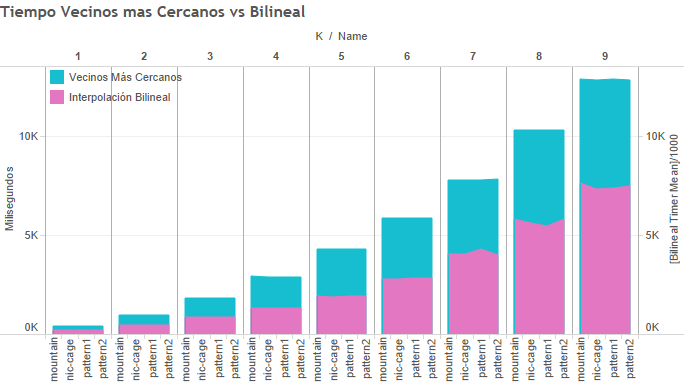
\includegraphics[scale=0.8]{BI-Time-knn_vs_bilineal.png}
\caption{Comparando tiempo de cómputo del método de Vecinos mas Cercanos con el de Bilineal}
\label{fig:BI-time-knn_vs_bilineal}
\end{figure}
\begin{figure}[H]
\centering
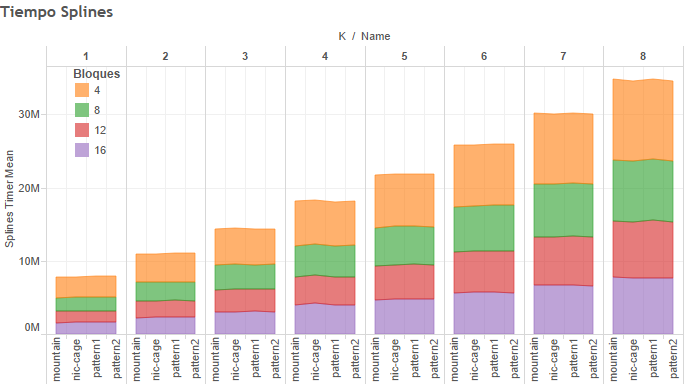
\includegraphics[scale=0.8]{BI-Time-Splines.png}
\caption{Tiempo de cómputo interpolación por splines segun el tamaño de bloque}
\label{fig:BI-time-Splines}
\end{figure}
Por lo que se puede ver en la Figura \ref{fig:BI-time-knn_vs_bilineal}, la hipótesis sobre el método de vecinos mas cercanos es acertada. Hay que notar que en la implementación la diferencia entre procesar un punto nuevo y mantener un punto viejo es nula en complejidad temporal, mantener un punto viejo es simplemente copiar los datos de ese punto original a su lugar correspondiente en la imagen agrandada en $O(1)$, y calcular un punto nuevo es básicamente ver que punto de los originales esta mas cerca, y como solo hay 4 posibles candidatos como mucho, esto se reduce también a $O(1)$, por lo tanto el tiempo de computo va a verse afectado únicamente por el tamaño de la imagen agrandada, y este valor esta representado por $k$, y cuando $k$ crece, crece cuadraticamente la cantidad de píxeles a calcular, ya que $k$ actúa a lo ancho y alto.\smallbreak
En esa misma Figura \ref{fig:BI-time-knn_vs_bilineal} se puede ver que la segunda hipótesis fue también acertada, esto se debe que, para generar cada valor nuevo (nuevo píxeles) se realiza una sola operación, por lo tanto el tiempo va a terminar dependiendo de cuantos píxeles hay que generar, al igual que el caso anterior, depende de $k$ y afecta cuadraticamente a la cantidad de píxeles a generar.\smallbreak

El segundo método tarda menos que el primero ya que el segundo solo realiza una operación por píxel a generar, y el primero, por cada píxel a generar, debe calcular su distancia con al menos 2 píxeles y como mucho 4. Por lo tanto cuesta mas temporalmente calcular usando Vecinos mas cercanos que Bilineal. \smallbreak

Por ultimo en la Figura \ref{fig:BI-time-Splines} se puede ver los datos recopilados sobre el método de Interpolación por Splines, y lo que se puede ver es que la variación de $k$ va a afectar al tiempo de computo de forma potencial. Al analizar el algoritmo de la implementación uno ve a simple vista que se compone por dos ciclos $for$ anidados que dependen del tamaño de la imagen original y del tamaño de bloque, estos $for$ van a ir iterando por cada bloque a procesar, entonces cuanto mas grande sea el bloque, menos iteraciones realizaran (porque entrara menos bloques en total). Luego, por cada bloque el algoritmo primero interpolara primero entre los píxeles viejos que se mantuvieron (ahora estarán con k píxeles de distancia entre ellos) de forma horizontal y luego de forma vertical, por lo tanto hará una función interpoladora por linea y columna con puntos viejos, y evaluara la función en los puntos nuevos a calcular. El tiempo que lleva calcular estos polinomios va a ser afectado solamente por el tamaño de bloque $B$, ya que siendo el bloque mas grande abarcara mas puntos originales, por lo tanto crecerá el sistema de ecuaciones a resolver para calcular el polinomio de interpolación, mas específicamente crecerá la matriz a la que luego se le aplicara eliminación gaussiana que cuesta $O(n^2)$ calcular, siendo n el ancho de la matriz (igual la matriz es cuadrada en este caso), ese n va a ser $B$ ya que representa la cantidad de puntos originales que abarca un bloque.\par
Ahora ya tendríamos procesados los píxeles que se encuentran entre los píxeles que se mantuvieron vertical y horizontalmente, luego se procede a ir fila por fila y crear un polinomio de interpolación por splines para cada una, generando de esa forma los píxeles faltantes, por lo tanto nuevamente el costo que llevara generar el polinomio de interpolación se vera afectado solo por el tamaño de bloque $B$ de forma cuadrática.\par
Sabiendo todo este procedimiento se llega a la conclusión que $k$ solamente afecta inmediatamente luego de generar los polinomios de interpolación por splines, al momento de evaluar la función generada en los píxeles faltantes (los nuevos), aquí es donde entra en juego $k$ ya que va a modificar cuantas evaluaciones de la función hay que hacer, ya que, como vimos antes, incrementara cuadraticamente la cantidad de píxeles nuevos.\par
Todo esto quiere decir que la complejidad temporal se ve afectada independientemente por $B$ y por $k$. Y esto se refleja muy acordemente en la Figura \ref{fig:BI-time-Splines}, ya que para todos los tamaños de bloque el crecimiento con respecto a $k$ es el mismo.\par\smallbreak

Las complejidades son aproximadas\par\smallbreak

Algo muy importante que se puede ver para todos los métodos es que la información de la imagen no afecta al tiempo de computo del algoritmo, por lo tanto acertamos también en esa hipótesis.\smallbreak

Por ultimo vamos a poder ver como se comparan los tiempos entre todas las pruebas que realizamos en esta sección:

\begin{figure}[H]
\centering
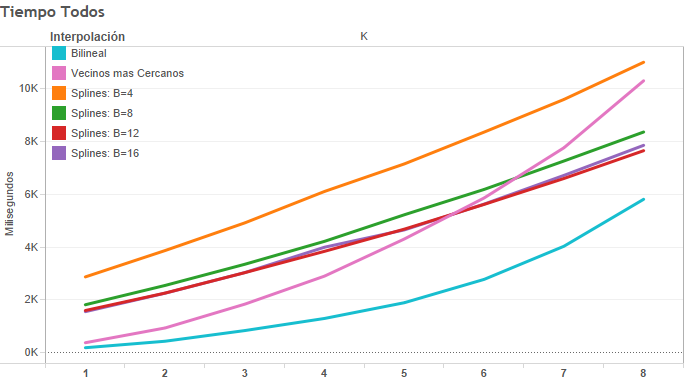
\includegraphics[scale=0.8]{BI-Time-All.png}
\caption{Tiempo de cómputo de todos los casos de experimentación}
\label{fig:BI-time-Splines}
\end{figure}

Se puede ver que el método de Zoom utilizando Interpolación por splines puede tener un menor costo temporal a medida que $k$ se agranda, esto sucede porque a medida que $B$ crece, entran menos cantidad de bloques en la imagen original, por lo tanto el tiempo de calculo se va reduciendo. Hay que tener en cuenta igual que, a medida que $k$ se agranda, el error también se va agrandando, y utilizando un $k$ muy grande ya la imagen deja de ser coherente, por lo tanto el zoom por interpolación bilineal va a ser el mas útil de usar, en términos de tiempo de computo, para la mayoría de los casos en los que se utilice.

\section{Conclusión}

Lo que primero pudimos concluir de la experimentación fue que la eficiencia del método depende fuertemente del tipo de imagen. Si bien las métricas nos dicen cuál fue el error promedio, o cuán parecida es la imagen con zoom a la que debería ser, esto no quita que dos imágenes tengan el mismo error numéricamente, y sin embargo una de ellas tenga errores mucho más visibles que la otra. En primer lugar, dos imágenes pueden tener el mismo error cuadrático medio, pero si una de ellas tiene un error muy concentrado y la otra tiene el error más disperso, visualmente la primera será peor. En segundo lugar, la percepción visual del error depende de la composición de la imagen: para imágenes de rostros, por ejemplo, los errores en los ojos son muy notorios visualmente, ya que naturalmente se conoce qué forma deberían tener, y por lo tanto al encontrar irregularidades, por más pequeñas que sean, son muy notorias.

Vimos que para las imágenes de paisajes y de rostros, tanto el método de interpolación bilineal como el de vecinos más cercanos son muy similares en cuanto al error al interpolar, mientras que para las imágenes geométricas la diferencia es mucho más notoria. Se puede ver, sin embargo, que interpolación bilineal consistentemente alcanza un menor error.

Por otra parte, el método de interpolación bilineal y el de splines se comportan (en cuanto a las métricas) de manera muy similar para las imágenes de paisajes y rostros, incluso variando ampliamente la cantidad de bloques. En cuanto a las geométricas, bilineal se comporta levemente mejor. Como bilineal tiene un mejor tiempo que vecinos más cercanos y que splines (con un $k$ no muy grande), si se debe ampliar una imagen cuyo tipo se desconoce, el análisis cuantitativo nos diría que el mejor método es el bilineal. Sin embargo, al efectuar el análisis cualitativo, splines aumenta las imágenes de manera que el error es menos perceptible para el ojo humano, y por lo tanto no podemos concluir que un método sea superior al otro para todo caso. Es importante entonces, antes de elegir el algoritmo a utilizar, considerar la composición de la imagen. Para imágenes geométricas, el mejor método es el bilineal, mientras que para imágenes de rostros, donde los errores son muy visibles, es preferible pagar un costo más alto en tiempo de cómputo y utilizar splines. Para imágenes de paisajes, ambos métodos son efectivos, pero si se desea ahorrar en tiempo de cómputo se puede optar por utilizar interpolación bilineal.

Hay que tener en cuenta que el hecho de usar un $k$ lo suficientemente grande va a generar una imagen demasiado incoherente, por lo tanto este parámetro va a depender estrictamente del uso que se le quiera a dar a la imagen de salida, si por ejemplo uno genera la imagen para que se vea desde muy lejos (propagandas de autopista por ejemplo) uno va a poder utilizar un $k$ grande sin mayores problemas, y al utilizar un $k$ así de grande va a ser mas recomendable utilizar interpolación por splines, ya que tiene un menor costo temporal con $k$ grandes, y además el error perceptible visualmente va a ser menor si se utiliza además un tamaño de bloque grande (que entren como mucho 4 bloques en la imagen original) ya que no solo beneficia al costo temporal, sino que genera menos anomalías perceptibles a la vista humana.
Si se va a utilizar un $k$ menor a 9 aproximadamente, va a ser mas rápido utilizar el zoom con interpolación bilineal, y además la diferencia entre los errores no es tan extensa como para justificar utilizar splines (que provoca menos errores perceptibles).

\section{Referencias}
\begin{itemize}
\item Apuntes teóricos de la cátedra.
\item Numerical analysis - Richard L. Burden J. Douglas Faires - 2011
\end{itemize}

\end{document}